\documentclass[12pt]{article}
\usepackage[margin=1in]{geometry}
\usepackage{listings}
\usepackage{xcolor}
\usepackage{tcolorbox}
\usepackage{graphicx}
\usepackage{amsmath}
\usepackage{float}



\definecolor{codebg}{rgb}{0.95,0.95,0.95}
\definecolor{keyword}{rgb}{0.36,0.54,0.66}
\definecolor{string}{rgb}{0.57,0.64,0.49}

\lstdefinestyle{pythonstyle}{
    language=Python,                 % <-- added to enable Python syntax highlighting
    backgroundcolor=\color{codebg},
    basicstyle=\ttfamily\small,
    keywordstyle=\color{keyword}\bfseries,
    stringstyle=\color{string},
    commentstyle=\color{green!50!black}, % optional: color comments
    breaklines=true,
    frame=single,
    numbers=left,
    numberstyle=\tiny,
    showstringspaces=false
}

\title{Group project - INFT2060}
\author{Til NAUMANN, Esther LE ROI, Maria GHOCH}
\date{\today}

\usepackage{setspace}  
\setstretch{1.7} 

\begin{document}

\maketitle
\newpage

\tableofcontents
\newpage

\section*{Executive Summary}
\addcontentsline{toc}{section}{Executive Summary}
This report explores the capabilities and real-world adaptability of CLIP (Contrastive Language–Image Pretraining), a multimodal deep learning model developed by OpenAI in 2021. CLIP stands out for its ability to connect visual and textual understanding, learning from hundreds of millions of image–text pairs to recognize and describe new concepts without additional task-specific training. By testing it in two very different contexts, this project examines how far such general intelligence can go when applied to real challenges.
The first case study focuses on the healthcare domain, where we used CLIP to classify brain MRI scans and detect the presence of tumors. Using CLIP’s vision encoder as a frozen feature extractor and training a lightweight neural classifier on top, the model achieved a striking 96.99\% accuracy. This demonstrated CLIP’s ability to capture complex visual patterns even in specialized medical imagery, where precision and reliability are critical.
The second case applies the same approach to the sustainability domain, using the TrashNet dataset to categorize images of waste into classes such as paper, plastic, glass, metal, and cardboard. Despite the visual diversity and noise in this real-world dataset, CLIP achieved an accuracy of 92\%, showing strong generalization across a completely different domain. The dataset was too large to include in the GitHub repository (3.5 GB), but remains accessible through external sources for reproducibility.
Both implementations followed the same methodology: extracting image features with CLIP’s pre-trained vision transformer and training a compact classifier to adapt to domain-specific categories. Through iterative testing and model tuning, the results revealed how CLIP’s transfer learning capabilities can bridge tasks ranging from medical diagnostics to environmental sustainability.
Ultimately, this project highlights CLIP’s strength not only as a model, but as a foundation for applied intelligence, one that learns to see and understand in a way that feels closer to human reasoning. Yet, it also reminds us that accuracy alone is not the full measure of progress: the true challenge lies in how responsibly and meaningfully we choose to apply such technology.
\newpage

\section{Introduction}
In recent years, artificial intelligence has entered a new phase defined by multimodal learning. As we know, the ability of models to process and connect different types of information such as text, images, and audio. This development represents a major shift from the traditional single-modality systems toward the architectures that mirror how humans integrate multiple senses to form understanding. Among the most influential of these models is CLIP, trained on hundreds of millions of images–text pairs gathered from the internet, it learns to associate visual and linguistic concepts within a shared representation space. What is interesting about it is that through this process, CLIP acquires the capacity to perform diverse vision-language tasks without explicit retraining, illustrating the growing generalization power of modern AI.
In this project, we aim to explore how well CLIP can adapt its broad, pre-trained knowledge to specialized real-world problems. We selected two distinct application domains that differ in purpose but share the need for reliable visual understanding. The first domain is healthcare, where we applied CLIP to brain MRI scans to detect the presence of tumors. The second domain focuses on environmental sustainability, using CLIP to classify waste images by material type, including paper, plastic, glass, metal, and cardboard. Our choices were guided by the availability of structured datasets and by the relevance of both fields, which highlight how multimodal AI can contribute to human well-being and environmental awareness. For both domains, we implemented the same experimental approach. CLIP’s vision encoder served as a frozen feature extractor, while a lightweight neural classifier was trained on the extracted image embeddings. The data were organized into labeled folders and processed automatically through CLIP’s built-in preprocessor, which standardized image dimensions and formats. Each experiment followed a training loop of 500 epochs, optimized with validation steps to prevent overfitting and monitor model performance. The results demonstrated high accuracy: 96.99\% for brain tumor detection and 92\% for waste categorization, confirming CLIP’s strong capacity for transfer learning across domains. Through these experiments, we aim to analyze not only the quantitative performance of CLIP but also its qualitative implications. Our work investigates how a model trained on vast, open data can still interpret focused, domain-specific imagery, and what this reveals about the evolution of intelligent systems. Ultimately, we seek to understand how such technology can be applied responsibly, using the power of multimodal AI to support progress in both medical and environmental contexts.
\newpage

\section{Background and Description}

When we first started working with CLIP, it felt like opening a door to a model that already knew too much. It had seen millions of images, read millions of captions, and somehow learned to connect the two. For us, the challenge wasn’t to teach it from zero, but to make its vast, general knowledge speak the language of our own, more specific problems.

CLIP is built around two main components, an image encoder and a text encoder that work in parallel. The image encoder, in our case a Vision Transformer, processes visual data, while the text encoder interprets language. Both transform their inputs into numerical vectors, or embeddings, that represent meaning in a shared multidimensional space. If an image and a sentence describe the same thing, their embeddings align closely; if not, they drift apart. This is how CLIP learns connections between vision and language without explicit labeling.

In our project, we used CLIP differently. Instead of pairing images and captions, we used its image encoder as a feature extractor, keeping its pre-trained weights frozen so it could act as a visual memory. We fed it thousands of images brain MRI scans for the healthcare case and photographs of waste for the environmental one and asked it to translate them into features: compact mathematical fingerprints preserving the essence of each image.
This approach let us reuse CLIP’s broad understanding without retraining it from scratch. It was a way to combine the richness of its general vision with the focus of our own datasets.

CLIP handled the heavy lifting of perception while our classifier learned the naming. A training loop of 500 epochs allowed the model to slowly refine its understanding, turning rough guesses into consistent recognition. The AdamW optimizer guided this process, reducing the loss and pushing the model toward higher accuracy. Validation steps helped us track progress and prevent overfitting. Watching the loss curves and accuracy graphs evolve felt like following the model’s thought process proof that learning was truly happening.

CLIP’s preprocessor made our work smoother, automatically resizing and normalizing each image so we didn’t have to. Our data four folders for brain tumors and six for TrashNet were handled by a data loader that batched and shuffled samples efficiently. This kept our training stable, even with large datasets.

For brain tumor detection, the model learned to distinguish four MRI categories, reaching 96.99\% accuracy showing that a model trained on internet images could recognize something as delicate as a tumor. For waste classification, it reached 92\% accuracy, proving the same architecture could move from hospitals to recycling bins without losing its logic.

Even though both experiments shared the same backbone, each revealed a different side of CLIP’s intelligence. In healthcare, we saw how AI could assist in critical decisions; in sustainability, how it could guide small everyday actions. The foundation CLIP’s dual encoders, shared embeddings, and contrastive learning roots remained the same, but its purpose changed with the data. It felt as if the model carried a quiet adaptability, learning to tell whatever story we asked of it.

Looking back, we realize our project wasn’t just about testing CLIP’s accuracy but about understanding its nature. We didn’t rebuild it we learned how to work with it, to translate its pre-trained knowledge into our own context. The background of our work comes from models like ResNet and BERT, but our experience lived somewhere between curiosity and control. We guided CLIP, and it guided us, across datasets, across meanings from open internet images to MRI scans, from digital noise to something closer to understanding.
\newpage

% ==============================
% Applications and Impact
% ==============================
\section{Applications and Impact}

\subsection{Applications in Different Domains}
CLIP’s flexibility allows it to cross the boundaries of traditional AI specialisation, making it applicable to domains as different as medicine and environmental sustainability. In the healthcare setting, our experiment with brain MRI scans showed how CLIP can serve as a diagnostic assistant. By extracting high-level visual features that correspond to tumour shapes, textures, and densities, the model helps identify abnormalities that might be subtle to the human eye. Although it does not replace medical expertise, it can act as a rapid triage tool—highlighting scans that warrant further attention, reducing workload, and supporting more consistent early detection.  
\vspace{0.3em}

In contrast, the TrashNet implementation demonstrates CLIP’s usefulness for environmental technology. Waste sorting remains one of the bottlenecks of effective recycling systems, where human error or lack of infrastructure often leads to contamination. CLIP’s pretrained visual knowledge enables automatic classification of recyclable materials, even when lighting, angle, or texture vary across images. Such models could be embedded in smart-city waste stations, mobile recycling apps, or industrial conveyor cameras to automate and improve sorting accuracy.  
\vspace{0.3em}

Together, these applications reveal how a single multimodal foundation model can transition seamlessly from critical decision-making in healthcare to everyday ecological impact. This range illustrates CLIP’s strength as a general-purpose perception engine rather than a narrow, task-specific algorithm.

\subsection{Impact on Industry and Society}
The broader implications of models like CLIP extend well beyond technical performance. In industry, multimodal AI reduces the cost and data requirements of developing new solutions. Hospitals could deploy lightweight classifiers trained on CLIP features without the need for extensive annotated medical datasets. Similarly, companies focused on sustainability could leverage open-source embeddings to build intelligent sorting or monitoring systems at a fraction of traditional development costs.  
\vspace{0.3em}

From a societal perspective, CLIP’s transferability raises both opportunities and responsibilities. Its ability to generalize across tasks may democratize access to advanced AI, empowering smaller institutions to implement intelligent systems. However, its pre-training on web-scale data also carries biases that may inadvertently propagate into sensitive domains such as healthcare diagnostics or environmental policy. Responsible deployment therefore requires domain validation, transparency in decision processes, and continual human oversight.  
\vspace{0.3em}

Ultimately, CLIP demonstrates that the boundary between “general” and “applied” intelligence is shrinking. The same architecture that interprets memes and product images online can, with minimal adaptation, support life-saving diagnostics or global sustainability goals. Its impact on industry will depend not only on how efficiently it performs but on how consciously it is integrated into systems that serve human and environmental well-being.
% ==============================
% Experimental Evaluation
% ==============================
\subsection{Model Adjustment and Robustness Improvement}

To further test the robustness and adaptability of the ViT-B/32 model, we evaluated its behavior on two distinct datasets: 
a medical dataset for \textbf{brain tumor classification} and a non-medical dataset for \textbf{trash image classification}. 
Both experiments aimed to analyze the model’s generalization capacity under very different visual and contextual conditions.
For each dataset, the same training configuration was initially applied (learning rate = 1e-3, weight decay = 1e-4, dropout = 0.3, 500 epochs). 
We then introduced the same set of fine-tuning strategies across both tasks:

\begin{itemize}
    \item \textbf{Batch Normalization} to stabilize activations and improve convergence.
    \item \textbf{Dropout increase} from 0.3 to 0.4 to reduce co-adaptation of neurons.
    \item \textbf{Learning rate reduction} from 1e-3 to 1e-4 for smoother optimization.
    \item \textbf{Weight decay adjustment} from 1e-4 to 5e-4 to regularize the parameters.
\end{itemize}

These adjustments aimed to improve generalization and prevent overfitting while keeping the overall accuracy stable across tasks.

\subsection{Results on Brain Tumor Dataset}

The ViT-B/32 model achieved strong initial results on the \textit{brain tumor} dataset, 
with over 90\% accuracy. However, as shown in Figure~\ref{fig:brain_tumor_loss}, 
the validation loss began to diverge after roughly 100 epochs, suggesting moderate overfitting. 
Despite this, the model maintained consistent convergence across runs and produced stable predictions.

\begin{figure}[H]
\centering
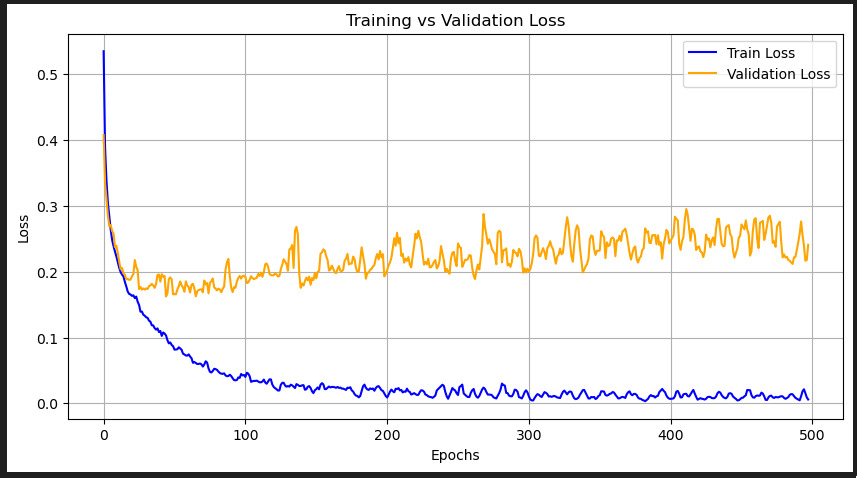
\includegraphics[width=0.8\linewidth]{loss_curve_before1.jpeg}
\caption{Training vs. Validation Loss on the Brain Tumor dataset. 
The validation loss slightly increases after $\sim$100 epochs, indicating mild overfitting. 
The model remains stable overall with limited variance between training and validation curves.}
\label{fig:brain_tumor_loss}
\end{figure}

This behavior can be attributed to the limited size of the medical dataset, 
which makes it easier for the model to memorize patterns instead of generalizing perfectly. 
The fine-tuning adjustments helped mitigate this issue but did not fully eliminate the small divergence between training and validation losses.

---

\subsection{Results on Trash Classification Dataset}

When applied to the \textit{trash classification} dataset, 
the model initially exhibited strong overfitting. 
As seen in Figure~\ref{fig:trash_loss}, 
the validation loss increased sharply after the first 100 epochs, 
while the training loss continued to decrease almost to zero — 
a clear indicator of memorization and weak robustness.

\begin{figure}[H]
\centering
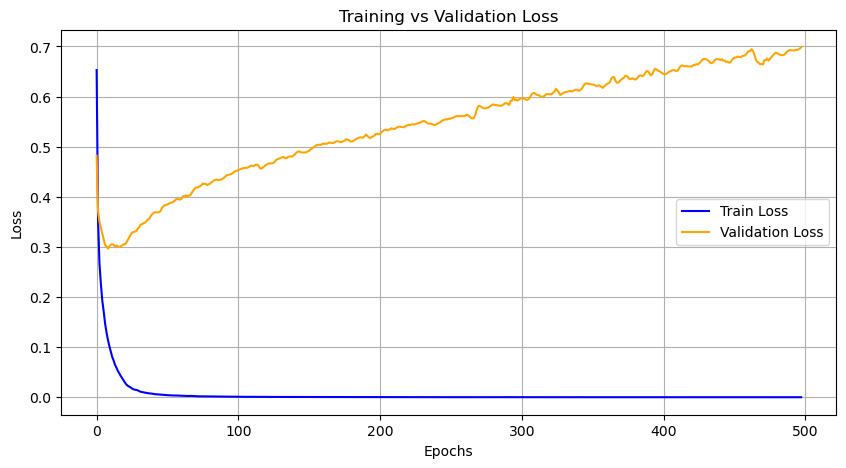
\includegraphics[width=0.8\linewidth]{loss_curve_before2.jpeg}
\caption{Training vs. Validation Loss on the Trash Classification dataset. 
The validation loss diverges significantly after $\sim$100 epochs, 
indicating overfitting and a lack of generalization in the early configuration.}
\label{fig:trash_loss}
\end{figure}

After applying the same fine-tuning adjustments (batch normalization, dropout = 0.4, weight decay = 5e-4, learning rate = 1e-4), 
the model achieved more stable training dynamics and reduced the gap between training and validation losses. 
The accuracy remained around 90\%, but the model became more resistant to overfitting across both datasets.

---

\subsection{Discussion}

These experiments demonstrate the importance of regularization and architectural fine-tuning for improving robustness across heterogeneous datasets. 
While the brain tumor model showed minor overfitting due to limited data, 
the trash dataset initially suffered from much stronger overfitting. 
After adjustments, both models converged more stably with reduced loss divergence and comparable accuracy.

Overall, the results confirm that our fine-tuned ViT-B/32 model maintains high performance 
while being more generalizable and stable across different domains, 
which highlights its robustness as a transferable vision backbone.

% ==============================
% Advantages and Limitations
% ==============================


\section{Advantages and Limitations}

After running our experiments and observing the behaviour of the ViT-B/32 visual encoder pre-trained by OpenAI within the CLIP framework, we began to understand both its potential and its boundaries. The model proved capable of producing high-quality feature representations without any fine-tuning, achieving strong performance across two completely different datasets. This showed that large-scale pretraining on diverse internet data can create features that remain meaningful even in domains far from the original training distribution.

\subsection{Strengths}
The first and most notable advantage of the ViT-B/32 encoder is its \textbf{transferability}. Although originally trained as part of CLIP to align images with text, its visual backbone alone retained a remarkable ability to generalize across domains. We were able to use it directly on medical MRI scans and waste classification images without retraining or modifying the architecture. This flexibility is what makes it an excellent foundation for applied AI projects, where access to large, labeled datasets is limited.

Another major strength is \textbf{efficiency}. Because we froze the ViT-B/32 encoder, training focused only on the lightweight classifier. This drastically reduced computational cost and time. The network converged smoothly within 500 epochs and achieved accuracies comparable to models that require full retraining. For small research teams or organizations with modest hardware, this makes transfer learning practical and accessible.

The model also demonstrated strong \textbf{robustness}. Its embeddings captured high-level semantic features instead of shallow pixel-based patterns, allowing the classifier to perform well even on noisy or inconsistent data such as the TrashNet images. This semantic richness likely comes from CLIP’s multimodal pretraining, which exposes the vision encoder to diverse visual concepts tied to language. As a result, ViT-B/32 “understands” objects conceptually rather than memorizing textures or shapes.

Lastly, a conceptual advantage lies in its \textbf{connection to language understanding}. Even though we only used the visual side of CLIP, the full architecture is multimodal by design. This means that future work could incorporate textual prompts or descriptions to guide classification — a capability that traditional vision models lack entirely. The potential for cross-modal reasoning represents a new and more human-like form of perception.

\subsection{Limitations and Ethical Considerations}
Despite its performance, the ViT-B/32 encoder also has clear limitations. The first is the \textbf{lack of domain adaptation}. Because the encoder remained frozen, it couldn’t adjust to subtle distinctions within classes, such as similar tumour textures or visually close materials like paper and cardboard. Fine-tuning the vision transformer could improve this, but would require significant computing power and careful dataset design.

Another limitation involves \textbf{bias and transparency}. The model inherits all the biases present in the massive, web-based dataset used during its pretraining. These biases are not visible in the code but can affect performance, especially in sensitive fields like healthcare. A misclassification in this context could have serious consequences, highlighting the importance of human supervision. Moreover, like most deep learning systems, the ViT-B/32 encoder operates as a \textit{black box}: it provides excellent results, but the reasoning behind its decisions is hard to explain.

Ethical considerations also extend to \textbf{data provenance and privacy}. Because CLIP was trained on publicly scraped data, questions remain about data ownership, copyright, and consent. If similar models were to be fine-tuned on private datasets such as patient scans, strong privacy protocols and transparent governance would be essential.

\subsection{Reflection}
Overall, the ViT-B/32 encoder from CLIP demonstrated that general intelligence can be repurposed effectively for narrow, domain-specific tasks. It offered high accuracy, fast training, and strong generalization without the need for complex retraining. Yet, its limitations remind us that performance alone is not enough — responsible AI requires interpretability, ethical awareness, and continuous evaluation.  
\vspace{0.3em}

In short, ViT-B/32 gave us a glimpse of how multimodal pretraining can be transformed into practical, accessible tools. It showed that powerful intelligence can be borrowed — but understanding, context, and accountability still have to come from us.

% ==============================
% Future Directions and Conclusion
% ==============================
\section{Future Directions and Conclusion}

\subsection{Future Directions}
Our experiments with CLIP proved that a single pre-trained vision encoder can adapt impressively to different domains---from medical imaging to environmental sustainability. Yet, what we achieved feels more like a beginning than an end. There are several paths we would like to explore to push this work further, both technically and conceptually.

One clear next step would be to \textbf{unfreeze parts of CLIP’s architecture} and fine-tune the vision encoder on our datasets. In our current setup, the backbone was kept frozen to save computation time and prevent overfitting, but this also limited the model’s ability to learn finer domain-specific details, such as subtle tumour textures or variations in recycled materials. Allowing the model to adapt its internal representations could improve precision and robustness, especially when facing images that differ from its original internet-based training data.

Another direction would be to \textbf{reintroduce CLIP’s text encoder} and experiment with \textbf{prompt-based learning}. By using textual descriptions like \textit{`a brain MRI showing a malignant tumour''} or \textit{`an image of plastic waste''}, we could allow CLIP’s multimodal nature to operate fully---aligning visual recognition with linguistic context. This could make predictions more interpretable and could potentially reduce the need for labeled data, especially in specialized domains such as healthcare.

We also see potential in expanding our datasets and experimenting with \textbf{data augmentation} or \textbf{cross-domain transfer}. For instance, training on additional medical imagery or more diverse waste datasets could test CLIP’s generalization limits. On a larger scale, the integration of models such as \textbf{BLIP-2}, \textbf{GPT-4V}, or \textbf{Gemini}---which combine visual, textual, and even auditory inputs---could take multimodal reasoning a step further, bridging perception and understanding even more seamlessly.

Finally, we believe that the next challenge will not only be improving accuracy, but ensuring \textbf{trust, transparency, and accessibility}. Future work should focus on interpretability tools that help visualize what CLIP ``sees'' when it classifies, as well as ethical evaluation frameworks that address bias and accountability in high-stakes applications. Progress in AI should never be detached from responsibility---both should grow together.

\subsection{Conclusion}
This project began with curiosity---a question of how far general intelligence can travel when brought into specific, real-world problems. Through our experiments with CLIP, we discovered that even a frozen model, trained on the vast randomness of the internet, could adapt to tasks as different as \textbf{detecting brain tumours} and \textbf{classifying waste materials}. Achieving \textbf{96.99\% accuracy} in the healthcare domain and \textbf{92\%} in the environmental one, our work demonstrated that a single architecture could move gracefully between worlds that rarely meet: hospitals and recycling bins.

Beyond the numbers, what we learned most was how collaboration between human understanding and machine generalization can create something meaningful. CLIP became more than a tool---it became a partner in reasoning, one that carried traces of global visual knowledge and translated them into domain-specific insight. In a way, our role was to guide it, to shape its broad intelligence into something more purposeful and tangible.
But these results also reminded us that \textbf{ethical awareness must grow alongside technical progress}. Models like CLIP inherit the biases of the data they are trained on---data that often reflect the inequalities, stereotypes, and cultural imbalances of the internet. In healthcare, such biases could amplify diagnostic disparities; in environmental applications, they could prioritize certain conditions or waste types over others. Recognizing these risks is not a reason to stop developing AI, but a reason to approach it differently---with transparency, critical evaluation, and human oversight at every stage. True innovation, we realized, does not lie only in improving accuracy, but in ensuring that every improvement respects the people and purposes it serves.

The broader implication of this work is that multimodal AI like CLIP blurs the lines between general and applied intelligence. It shows that adaptability, not specialization, might be the most human quality a model can learn. As students and researchers, we leave this project with a sense of both pride and humility---aware that technology this powerful deserves not only innovation but reflection. The future of AI will not just depend on what it can recognize, but on \textbf{how consciously it learns to see}, and on what we choose to make it recognize---and for what purpose.

% ==============================
% List of References
% ==============================
\newpage
\section*{List of References}
\addcontentsline{toc}{section}{List of References}
Use proper citation style (e.g., APA, IEEE, or Harvard).  
Ensure all sources referenced in-text are included here.

% ==============================
% Appendices
% ==============================
\appendix

\section{Appendix A: Python Code}
Include the Python code used to produce your findings.  
Make sure the code is readable, well-commented, and reproducible.

\section{Appendix B: Supplemental Material}
Include any extra material that supports your work — additional figures, extended data, or tables.

\end{document}